\documentclass[dvipdfmx]{jarticle}
\usepackage{url}
\usepackage{graphicx}
\usepackage[top=30truemm,bottom=30truemm,left=25truemm,right=25truemm]{geometry}


\begin{document}
\begin{titlepage}
    \begin{center}
        {\huge データベース 課題3レポ―ト}
        \vspace{180pt}\\
        \begin{tabular}{rl}
            氏名 & 山久保孝亮\\
            所属 & 大阪大学基礎工学部情報科学科ソフトウェア科学コース\\
            メールアドレス & u327468b@ecs.osaka-u.ac.jp\\
            学籍番号 & 09B22084\\
            提出日 & \today\\
        \end{tabular}
    \end{center}
\end{titlepage}
\section{課題1}
\subsection{課題内容}
5人以下の学生が履修している科目の科目名とその科目を履修している学生数を求めよ
\subsection{SQLの問い合わせ文}
課題1の結果を返すためのSQLの問い合わせ文は以下の図1のようになる.\\
\begin{figure}[h]
    \centering
    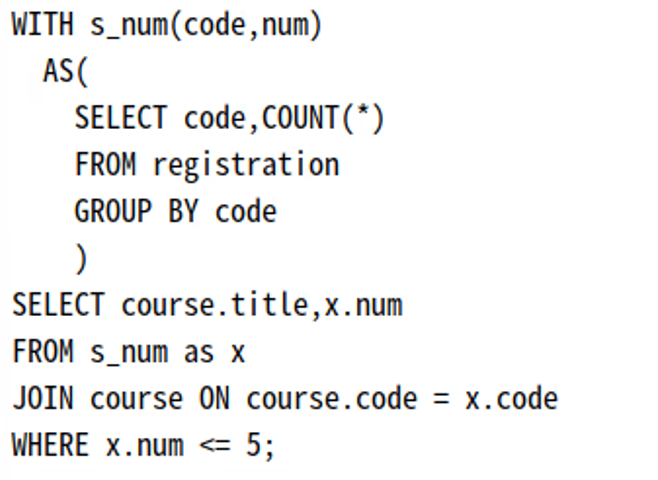
\includegraphics[width=7cm]{sql1.png}
    \caption{課題1のSQLの問い合わせ文}
\end{figure}
\subsection{SQL文の解法}
課題1では最終的に科目名と受講生の人数を出力する必要がある.
\\科目名に関してはcourseのtitleを参照すればよいが,受講生の人数を表すカラムが存在しないので,GROUP BY を使用し各codeごとにグループ表を作成する.その
個数をCOUNT(*)を使ってnumとして計算する.これにより,各codeの表の行数を数えることができ,それはそのcodeの受講人数を表す.\\
上記の処理をWITHを用いて行うが,処理後に作成された表をs\_numとした.\\
最終的に出力するのはs\_numのカラムのnumとcourseのカラムのtitleであるが,これらを連結する必要がある.したがって,それぞれの表に共通するカラムである
codeをJOINで結合する.\\
また,課題内容より,表示するのは受講生が5人以下の科目のみであるためWHEREにおいてnumが5以下という条件をつけた.
\clearpage
\subsection{SQL文の問い合わせ結果}
問い合わせの結果は以下の図2のようになる.\\
\begin{figure}[h]
    \centering
    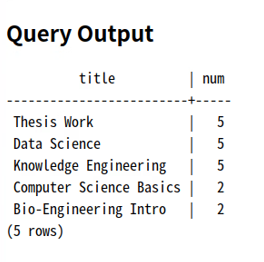
\includegraphics[width=4cm]{sqlresult1.png}
    \caption{課題1の問い合わせ結果}
\end{figure}
\subsection{mongoGBの問い合わせ文}
課題1の結果を返すためのmongoGBの問い合わせ文は以下の図3のようになる.\\
\begin{figure}[h]
    \centering
    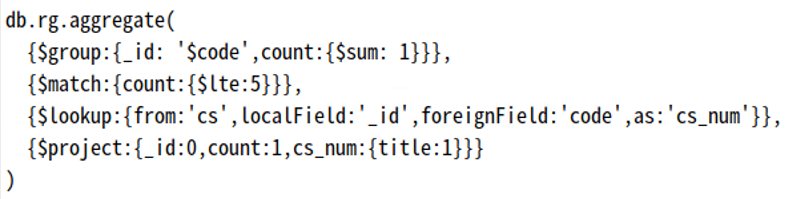
\includegraphics[width=10cm]{mongo1_code.png}
    \caption{課題1のmongoGBの問い合わせ文}
\end{figure}
\subsection{mongoGBの解法}
課題1のmongoGBの問い合わせ文は,1.2のSQL文から作成した.rgに対してaggregateを行った.各ステージの処理の詳細を以下で述べる.
\begin{enumerate}
    \item \$groupステージでは,1.2のSQLにおけるWITH内の処理を行っている.具体的には,codeごとにグループ表を作り,countにはそれぞれの表の行の数
    だけ1を足す.これにより,countが各codeごとの行数,即ち各講義の受講生の人数を表す.また,codeは\_idという名称になっている.
    \item \$matchステージでは,1.2のSQLにおけるWHEREの処理を行っている.具体的には,1で求めたcountが5以下のもののみを選択している.
    \item \$lookupステージでは,1.2のSQLにおけるJOINの処理を行っている.具体的には,1,2で求めた受講生が5人以下の講義のみのグループ表とcsを結合
    している.csとグループ表では,共通のフィールドはcodeと\_idであるため,それらによって結合を行っている.結合後の表はcs\_numという名称にした.
    \item \$projectステージでは,表示するフィールドの内容を指定している.\_idは明示的に0にしないと表示されるため0としている.これは,以下の課題でも同様
    である.また,課題内容より,表示するものは科目名と受講生の人数なので3で求めたcs\_numのフィールドであるtitleとnumを1とした.
\end{enumerate}
\subsection{mongoGBの問い合わせの結果}
問い合わせの結果は以下の図4のようになる.
\begin{figure}[h]
    \centering
    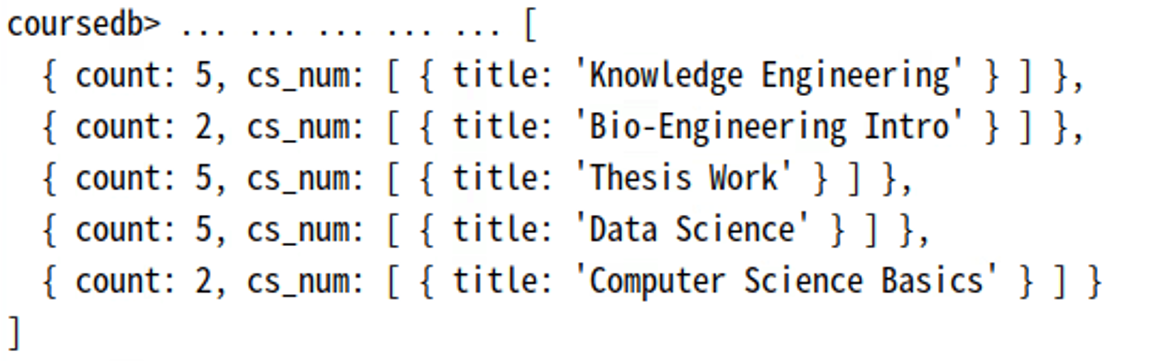
\includegraphics[width=8cm]{mongo1_result.png}
    \caption{課題1のmongoGBの問い合わせ結果}
\end{figure}
\section{課題2}
\subsection{課題内容}
教室が空値である科目の科目名とその科目を履修している学生の学生名を求めよ
\subsection{SQLの問い合わせ文}
課題2の問い合わせに答えるためのSQL文は以下のとおりである.
\begin{figure}[h]
    \centering
    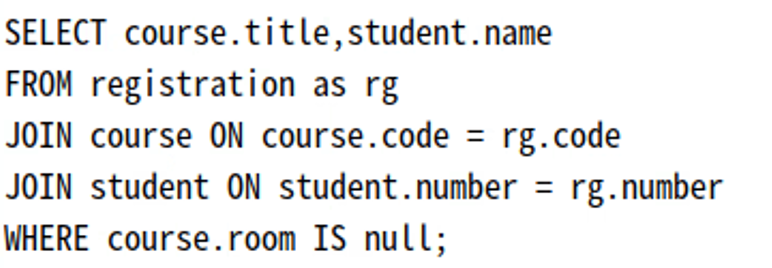
\includegraphics[width=5cm]{sql2.png}
    \caption{課題2のSQLの問い合わせ文}
\end{figure}
\subsection{SQL文の解法}
課題2では最終的に科目名と生徒名を出力する必要がある.\\
科目名はcourseに,生徒名はstudentテーブルに存在する.課題内容より,その科目を履修している学生名を表示しなければならないので,registrationテーブルと
前述の二つのテーブルをJOINを用いて結合する.\\
また,課題内容より,教室が空値である科目を選ぶ必要があるのでWHEREではcourseテーブルのroomがnullであるという条件をつけた.
\clearpage
\subsection{SQL文の問い合わせ結果}
問い合わせの結果は以下の図2のようになる.\\
\begin{figure}[h]
    \centering
    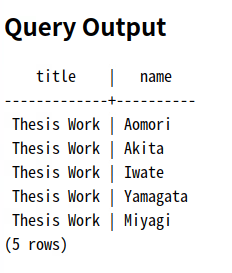
\includegraphics[width=4cm]{sqlresult2.png}
    \caption{課題1の問い合わせ結果}
\end{figure}
\subsection{mongoGBの問い合わせ文}
課題2の結果を返すためのmongoGBの問い合わせ文は以下のとおりである.\\
\begin{figure}[h]
    \centering
    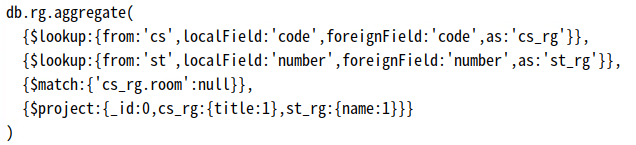
\includegraphics[width=8cm]{mongo2_code.png}
    \caption{課題2のmongoGBの問い合わせ文}
\end{figure}
\subsection{mongoGBの解法}
課題2のmongoGBの問い合わせ文も,2.2のSQL文から作成した.rgに対してaggregateを行った.各ステージの処理の詳細を以下で述べる.
\begin{enumerate}
    \item 一つ目の\$lookupステージでは,2.2のSQLにおけるJOINの処理を行っている.共通するフィールドであるcodeを用いてcsとrgを結合し,cs\_rgという表
    を作成した.
    \item 二つ目の\$lookupステージでは,2.2のSQLにおけるJOINの処理を行っている.共通するフィールドであるcodeを用いてcsとstを結合し,st\_rgという表
    を作成した.
    \item \$matchステージでは,2.2のSQLにおけるWHEREの処理を行っている.roomフィールドがnullであるものを選択している.
    \item \$projectステージでは,表示するフィールドの内容を指定している.課題内容より,科目名を表すtitleと生徒名を表すnameを1としている.
\end{enumerate}
\subsection{mongoGBの問い合わせの結果}
問い合わせの結果は以下の図2のようになる.
\begin{figure}[h]
    \centering
    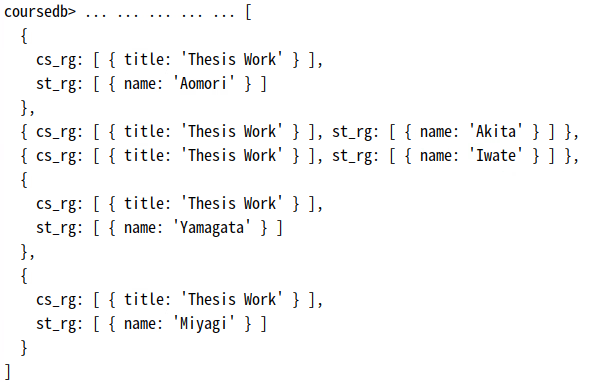
\includegraphics[width=7cm]{mongo2_result.png}
    \caption{課題2の問い合わせ結果}
\end{figure}
\section{課題3}
\subsection{課題内容}
必修の科目について科目ごとに科目名と成績の最高点およびその成績を取った学生名を求めよ
\subsection{SQLの問い合わせ文}
課題3の問い合わせに答えるためのSQL文は以下のとおりである.\\
\begin{figure}[h]
    \centering
    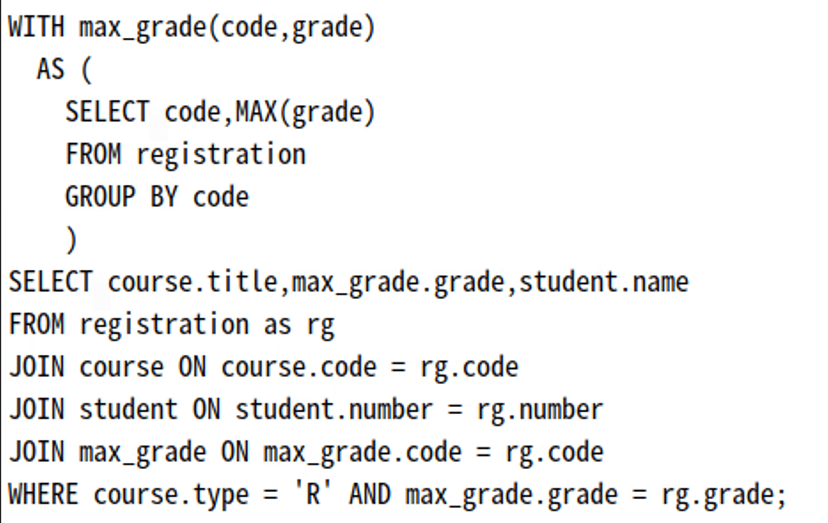
\includegraphics[width=12cm]{sql3.png}
    \caption{課題3のSQLの問い合わせ文}
\end{figure} 
\subsection{SQL文の解法}
課題3では最終的に科目名と最高点,学生名を出力する必要がある.\\
科目名はcourseテーブルのtitle,学生名はstudentテーブルのnameを参照すればよいが,各科目の最高点を表すカラムを含んだテーブルは存在しない.したがって,
WITH内でこの最高点を計算する処理を行う.WITHにより作成される表をmax\_gradeとし,カラムはcodeとgradeとした.GROUP BYを使ってcourseテーブルのcodeご
とにグループ表を作成し,courseテーブルのgradeの最大値をMAX()を使ってgradeとして選択する.これにより,このグループ表のgradeは各科目ごとの成績の最高
点を表すことができるようになる.\\
課題内容より,courseテーブル,studentテーブル,max\_gradeテーブルをregistrationテーブルとJOINを用いて結合する.これにより,必要な情報を含んだ表を
作成することができた.ただし,この表はregistrationテーブルのカラムgradeと,max\_gradeテーブルのカラムgradeを情報として持っている.\\
最後にWHEREの処理を記述する.まず必修の科目を選択するためにtypeが'R'と一致するものを選択する.この段階で上記の表は必修科目のみに絞り込むことができ
た.次に,各科目の成績の最大値を表すmax\_gradeテーブルのカラムgradeとregistrationテーブルのカラムgradeが一致している物を選択する.これにより,
それぞれのgradeが一致している物だけが,即ちregistrationテーブルのgradeが最大値のものだけが選択される.
\subsection{SQL文の問い合わせ結果}
問い合わせの結果は以下の図のようになる.\\
\begin{figure}[h]
    \centering
    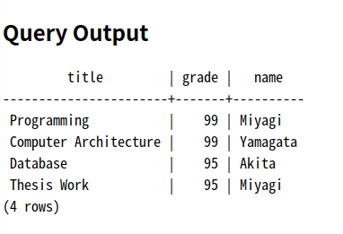
\includegraphics[width=4cm]{sqlresult3.png}
    \caption{課題3の問い合わせ結果}
\end{figure}
\subsection{mongoGBの問い合わせ文}
課題3の結果を返すためのmongoGBの問い合わせ文は以下のとおりである.\\
\begin{figure}[h]
    \centering
    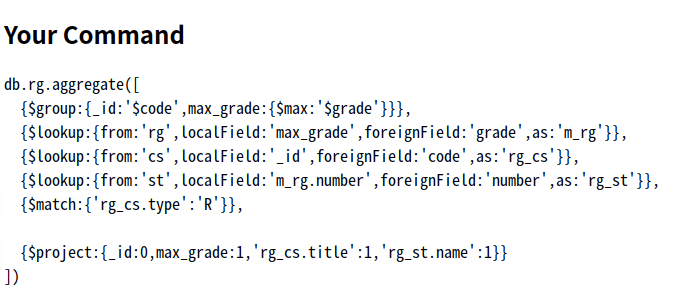
\includegraphics[width=8cm]{mongo3_code.png}
    \caption{課題3のmongoGBの問い合わせ文}
\end{figure}
\subsection{mongoGBの解法}
課題3のmongoGBの問い合わせ文も,3.2のSQL文から作成した.rgに対してaggregateを行った.各ステージの処理の詳細を以下で述べる.
\begin{enumerate}
    \item \$groupステージでは,3.2のSQL文におけるWITHの処理を行っている.具体的には,codeごとにグループ表を作り,max\_gradeにはgradeの最大値を格納
    する.また,codeは\_idという名称になっている.
    \item 一つ目の\$lookupステージでは,3.2のSQLにおけるJOINの処理を行っている.ここでは,1で作成したグループ表とrgを結合している.ここでrgと結合
    する理由としては,csとstとそれぞれ結合する際,共通するフィールドが存在しないためである.今回はgradeとmax\_gradeを共通するフィールドとして結合し
    ている.また,結合後の表はm\_rgとした.共通するフィールドとしてmax\_gradeを選んだ理由としては,各科目番号の成績の最大値のデータのみに絞り込むこと
    ができるためである.即ち,ここではJOINの処理だけでなくWHEREのANDの右側の処理も行っている.
    \item 二つ目の\$lookupステージでも,3.2のSQLにおけるJOINの処理を行っている.codeと\_idを用いてm\_rgとcsを結合し,rg\_csという表
    を作成した.
    \item 三つ目の\$lookupステージでも,3.2のSQLにおけるJOINの処理を行っている.codeと\_idを用いてm\_rgとstを結合し,rg\_stという表
    を作成した.
    \item \$matchステージでは,3.2のSQLにおけるWHEREの処理を行っている.typeフィールドが'R'であるものを選択している.これにより,必修の科目のみを選
    択することができる.
    \item \$projectステージでは,表示するフィールドの内容を指定している.課題内容より,成績の最大値を表すmax\_grade,科目名を表すtitle,生徒名を表す
    nameを1としている.
\end{enumerate}
\subsection{mongoGBの問い合わせの結果}
問い合わせの結果は以下の図3のようになる.
\begin{figure}[h]
    \centering
    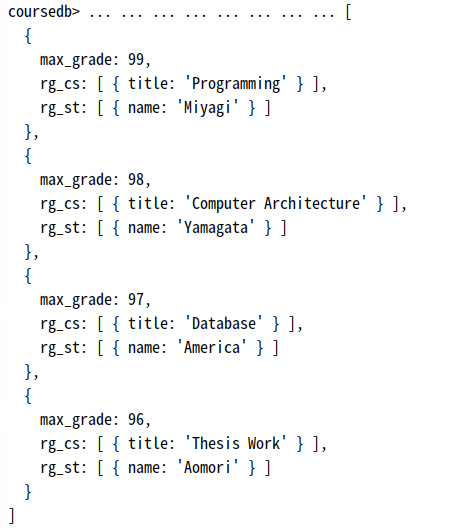
\includegraphics[width=6cm]{mongo3_result.png}
    \caption{課題3の問い合わせ結果}
\end{figure}
\section{感想}
今回の課題を通して難しく感じたことは,SQL文とMongoGBの結合の違いについてである.SQL文では3つ以上のテーブルを結合することができたが,MongoGBでは二つの
テーブルを結合することしかできない.したがって,結合するフィールドで工夫をする必要があった点が難しく感じた.
\end{document}